%%%%%%%%%%%%%%%%%%%%%%%%%%%%%%%%%%%%%%%%%%%%%%%%%%%%%%%%%%%%%%%%%%%%%%%%%%
%
%    phase1-GO.tex  (use only for General Observer and Snapshot proposals; 
%                      use phase1-AR.tex for Archival Research and
%                      Theory proposals use phase1-DD.tex for GO/DD proposals).
%
%    HUBBLE SPACE TELESCOPE
%    PHASE I OBSERVING PROPOSAL TEMPLATE 
%     FOR CYCLE 23 (2015)
%
%    Version 1.0, January 07, 2015.
%
%    Guidelines and assistance
%    =========================
%     Cycle 23 Announcement Web Page:
%
%         http://www.stsci.edu/hst/proposing/docs/cycle23announce 
%
%    Please contact the STScI Help Desk if you need assistance with any
%    aspect of proposing for and using HST. Either send e-mail to
%    help@stsci.edu, or call 1-800-544-8125; from outside the United
%    States, call [1] 410-338-1082.
%
%
%%%%%%%%%%%%%%%%%%%%%%%%%%%%%%%%%%%%%%%%%%%%%%%%%%%%%%%%%%%%%%%%%%%%%%%%%%%

% The template begins here. Please do not modify the font size from 12 point.

\documentclass[12pt]{article}
\usepackage{phase1}

%%%%%%%%%%%%%%%%%%%%%%%%%%%%%%%%%%%%%%%%%%%%%%%%%%%%%%%%%%%%%
%  PREAMBLE: sets up compiler modes, loads packages, defines macros, etc
%  Steve Rodney, 2012
%%%%%%%%%%%%%%%%%%%%%%%%%%%%%%%%%%%%%%%%%%%%%%%%%%%%%%%%%%%%%


%%%%%%%%%%%%%%%%%%%%
% COMPILER MODES
%%%%%%%%%%%%%%%%%%%%

% Changetext mode : highlight modified text in bold blue font
\newif{\ifchangetext}
\changetextfalse

%% Read in the -options.tex file (generated by the Makefile)
%%  to set the compile-mode options
\InputIfFileExists{\jobname-options}


%%%%%%%%%%%%%%%%%%%%%%%%%%%%%%%
% changetext  mode settings
%%%%%%%%%%%%%%%%%%%%%%%%%%%%%%%
\ifchangetext
  % Changed text is highlighted in bold, blue font 
  \newcommand{\change}[1]{{\bf \textcolor{blue}{#1}}}
\else
  % Changed text is indistinguishable
  \newcommand{\change}[1]{#1}
\fi


%%%%%%%%%%%%%%%%%%%%
% PACKAGES INCLUDED
%%%%%%%%%%%%%%%%%%%%
%\usepackage{wrapfig}
\usepackage{deluxetable} % deluxetable(*) environments
\usepackage{caption} % explicit figure captions
\usepackage{graphicx} % includegraphics commands
\usepackage{journalnames} % Astro Journal abbreviations
\usepackage{natbib}   % reference citations and bibliography
%\usepackage{amsmath}  % extended math symbols
\usepackage{verbatim} % verbatim text formatting
\usepackage{enumerate}% enumerated lists
%\usepackage{amssymb}  % extended symbols lib
\usepackage{url}      % url text formatting
\usepackage[usenames]{color}  % colored text
%\usepackage{multirow}  % muti-row table cells
%\usepackage{amsmath}  % extended equations lib (split)
%\usepackage{mathrsfs} % extended math fonts (mathscr)
%\usepackage{paralist} % inline enumeration (for Table ref lists)
%\usepackage{authblk}
\usepackage{multicol}
%\usepackage{subfig} % subfloats with independent captions
\usepackage{subcaption} % subfloats with independent captions
\usepackage{setspace} % switch from double to single spacing
\usepackage[none]{hyphenat} % Suppress the hyphenating
\usepackage{ulem} % for some underlining.
\usepackage{wrapfig}

%%%%%%%%%%%%%%%%%%%%%%%%%%%%%%%%%%%%%%%%%%%%%%%%%%%
% Redefine thebibliography for two-column formatting
% with the ``References'' title spanning the page
% http://tex.stackexchange.com/questions/20758/bibliography-in-two-columns-section-title-in-one
%   2013.02.22 : doesn't work with HST proposal sty files...?
%%%%%%%%%%%%%%%%%%%%%%%%%%%%%%%%%%%%%%%%%%%%%%%%%%%
\makeatletter
\renewenvironment{thebibliography}[1]
     {
  \begin{multicols}{2}[\section*{\refname}]%
      \@mkboth{\MakeUppercase\refname}{\MakeUppercase\refname}%
      \list{\@biblabel{\@arabic\c@enumiv}}%
           {\settowidth\labelwidth{\@biblabel{#1}}%
            \leftmargin\labelwidth
            \advance\leftmargin\labelsep
            \@openbib@code
            \usecounter{enumiv}%
            \let\p@enumiv\@empty
            \renewcommand\theenumiv{\@arabic\c@enumiv}}%
      \sloppy
      \clubpenalty4000
      \@clubpenalty \clubpenalty
      \widowpenalty4000%
      \sfcode`\.\@m}
     {\def\@noitemerr
       {\@latex@warning{Empty `thebibliography' environment}}%
      \endlist\end{multicols}}
\makeatother

%%%%%%%%%%%%%%%%%%%%%%%%%%%%%%%%%%%%%%%%%%%%%%%%%%%
% PDF mode settings : Auto-select eps or pdf figures 
% based  on the compiler used (i.e. latex vs pdflatex)
%%%%%%%%%%%%%%%%%%%%%%%%%%%%%%%%%%%%%%%%%%%%%%%%%%%
\ifx\pdfoutput\undefined
  \pdffalse
  \DeclareGraphicsExtensions{.eps,.ps}
\else
  \ifnum\pdfoutput=1
    % \pdftrue
    \DeclareGraphicsExtensions{.pdf,.png,.jpg}
  \else
    % \pdffalse
    \DeclareGraphicsExtensions{.eps,.ps}
  \fi
\fi


%%%%%%%%%%%%%%%%%%%%%%%%%%%%%%%
% AUTHOR-DEFINED MACROS
%%%%%%%%%%%%%%%%%%%%%%%%%%%%%%%
% General purpose usefulness:
\newcommand{\etal}{{et al.~}}                                             
\def\eg{{e.g.}}
\def\ie{{i.e.}}
\def\etc{{etc.}}
\newcommand{\lta}{\lesssim}                                               
\newcommand{\gta}{\gtrsim}                                                
\newcommand{\gt}{\gtsim}
%\newcommand{\kms}{\,\rm km\,s^{-1}}                                       

% Cosmology:
\def\Om{\ensuremath{\Omega_{\rm m}}}
\def\Ot{\ensuremath{\Omega_{\rm tot}}}
\def\Ob{\ensuremath{\Omega_{\rm b}}}
\def\OL{\ensuremath{\Omega_{\Lambda}}}
\def\Ok{\ensuremath{\Omega_{\rm k}}}
\def\om{\ensuremath{\omega_{\rm m}}}
\def\ob{\ensuremath{\omega_{\rm b}}}
\def\wo{\ensuremath{w_0}}
\def\wa{\ensuremath{w_{\rm a}}}
\def\lcdm{$\Lambda$CDM}
\def\LCDM{$\Lambda$CDM}
\def\wcdm{$w$CDM}
\def\Ho{\ensuremath{H_0}}
\def\DA{\ensuremath{D_A}}
\def\DL{\ensuremath{D_L}}

% Astronomy:
\def\arcsec{\ensuremath{^{\prime\prime}}} 
\def\kms{\ensuremath{{\rm km s}^{-1}}}
\def\hgpcq{\mbox{$h^{-3}$Gpc$^3$}}
\def\hmpcq{\mbox{$h^{-3}$Mpc$^3$}}
\def\perhmpcq{\mbox{$h^{3}$Mpc$^{-3}$}}
\def\hmpc{\mbox{$h^{-1}$Mpc}}
\def\hmpci{\mbox{$h$\,Mpc$^{-1}$}}
\def\mpc{\mbox{Mpc}}
\def\mpci{\mbox{Mpc$^{-1}$}}
\def\mpcq{\mbox{Mpc$^{-3}$}}
\def\Msun{\mbox{M$_{\odot}$}}
\def\Av{\mbox{$A_V$}}
\def\Rv{\mbox{$R_V$}}

% Supernovae : 
\newcommand{\tomas}{HFF14Tom}
\newcommand{\primo}{SN~Primo}
\newcommand{\CCSN}{CC\,SN}
\newcommand{\CCSNe}{CC\,SN}
\newcommand{\TNSN}{TN\,SN}
\newcommand{\TNSNe}{TN\,SNe}
\newcommand{\SNIa}{SN\,Ia}
\newcommand{\SNe}{SNe}
\newcommand{\SNeIa}{SN\,Ia}
\newcommand{\SNRz}{SNR($z$)}
\def\Mch{\mbox{M$_{\rm Ch}$}}
\def\Ni{\ensuremath{^{56}\mbox{Ni}}}
\newcommand{\dmfifteen}{\ensuremath{\Delta\mbox{m}_{15}}}
\newcommand{\deltamfifteen}{\ensuremath{\Delta\mbox{m}_{15}}}

% Missions:
\def\HST{{\it HST}}
\def\Hubble{{\it Hubble}}
\def\Hubbles{{\it Hubble's}}
\def\Spitzer{{\it Spitzer}}
\def\Chandra{{\it Chandra}}
\def\Herschel{{\it Herschel}}
\def\XMM{{\it XMM}}

% Institutions
\newcommand{\JHU}{Department of Physics and Astronomy, The Johns Hopkins University, Baltimore, MD 21218.}
\newcommand{\elsewhere}{St. Elsewhere University.}
\newcommand{\STScI}{Space Telescope Science Institute, Baltimore, MD 21218.}
\newcommand{\Berkeley}{Department of Astronomy, University of California, Berkeley, CA 94720-3411.}
\newcommand{\Riverside}{Department of Physics and Astronomy, University of California, Riverside, CA 92521.}
\newcommand{\WKU}{Department of Physics, Western Kentucky University, Bowling Green, KY 42101.}
\newcommand{\Copenhagen}{Dark Cosmology Centre, Niels Bohr Institute, University of Copenhagen, Juliane Maries Vej 30, DK-2100 Copenhagen, Denmark.}
\newcommand{\Arizona}{Department of Astronomy, University of Arizona, Tucson, AZ 85721.}
\newcommand{\SantaCruz}{Department of Astronomy and Astrophysics, University of California, Santa Cruz, CA 92064.}
\newcommand{\NotreDame}{Department of Physics, University of Notre Dame, Notre Dame, IN 46556.}
\newcommand{\TelAviv}{Department of Astrophysics, Tel Aviv University, 69978 Tel Aviv, Israel.}
\newcommand{\Rutgers}{Department of Physics and Astronomy, Rutgers, The State University of New Jersey, Piscataway, NJ 08854.}
\newcommand{\CfA}{Harvard/Smithsonian Center for Astrophysics, Cambridge, MA 02138.}
\newcommand{\Minnesota}{Department of Astronomy, University of Minnesota, 116 Church Street SE, Minneapolis, MN 55455, USA.}


%% Define a new 'leo' style for the url package 
%% that will use a smaller font.
% \def\UrlFont{\tt}
%\makeatletter
%\def\url@leostyle{%
%  \@ifundefined{selectfont}{\def\UrlFont{\sf}}{\def\UrlFont{\small\ttfamily}}}
%\makeatother
%%% Now actually use the newly defined style.
%\urlstyle{leo}


%%%%%%%%%%%%%%%%%%%%%%%%%%%%%%%
% Page Setup 
%%%%%%%%%%%%%%%%%%%%%%%%%%%%%%%
%  \renewcommand{\topfraction}{0.9}
%  \renewcommand{\bottomfraction}{0.9}
%  \renewcommand{\textfraction}{0.1}
%  \renewcommand{\floatpagefraction}{0.9}
%  \renewcommand{\dbltopfraction}{0.9}
%  \renewcommand{\dblfloatpagefraction}{0.9}



%%%%%%%%%%%%%%%%%%%%%%%%%%%%%%%%%%%%
%% Figure placement shortcuts    
%%%%%%%%%%%%%%%%%%%%%%%%%%%%%%%%%%%%

\newcommand{\figcaption}[1]{
\caption{{#1}}
}

\newenvironment{inlinefigure}{
\def\@captype{figure}
\noindent\begin{minipage}{0.999\linewidth}\begin{center}}
{\end{center}\end{minipage}\smallskip}

\newcommand{\insertfigwide}[2] {
\begin{figure*}
\begin{center}
\resizebox{\textwidth}{!}{\includegraphics{{#1}}}
\caption{{#2}}
\end{center}
\end{figure*}
}

\newcommand{\insertfiginline}[2] {
\begin{inlinefigure}
\begin{center}
\resizebox{\columnwidth}{!}{\includegraphics{{#1}}}
\figcaption{{#2}}
\end{center}
\end{inlinefigure}
}

\newcommand{\insertfigfloat}[2] {
\begin{figure}
\begin{center}
\resizebox{\columnwidth}{!}{\includegraphics{{#1}}}
\figcaption{{#2}}
\end{center}
\end{figure}
}

\newcommand{\insertfig}[2] {
\insertfigfloat{{#1}}{{#2}}
}

\newcommand{\insertfigdouble}[3] {
\begin{figure*}
\begin{center}
\resizebox{0.45\textwidth}{!}{\includegraphics{{#1}}}
\resizebox{0.45\textwidth}{!}{\includegraphics{{#2}}}
\figcaption{{#3}}
\end{center}
\end{figure*}
}


\newcommand{\insertfigend}[2] {
\newpage
%\vspace*{1.0in}
\begin{inlinefigure}
\begin{center}
\resizebox{\textwidth}{!}{\includegraphics{{#1}}}
\figcaption{{#2}}
\end{center}
\end{inlinefigure}
}


\begin{document}

%   1. SCIENTIFIC JUSTIFICATION
%       (see Section 9.1 of the Call for Proposals)
%
%
\justification          % Do not delete this command.
% Enter your scientific justification here. 

Over the past decade, the deep \HST\ Treasury surveys (GOODS, CANDELS,
CLASH) have proven to be the most effective programs for locating and
studying Supernovae (SNe) at high redshift.  These surveys have all
enabled ``piggyback'' SN searches,
which have collectively accumulated scores of SN detections that reach
to uniquely high redshifts
\citep{Riess:2007,Dahlen:2008,Graur:2014,Rodney:2014}.  Continuing in
this line of highly successful deep \HST\ surveys, the Hubble Frontier
Fields (HFF) director's discretionary program (PI:Lotz) now provides a
powerful new tool for the discovery of high-$z$ SNe.  What sets the
HFF program apart from previous surveys is the unique depth
of each visit; with $\sim$4 orbits per filter per epoch, we can reach
$m_{lim,3\sigma}(F160W)\approx27.9 (AB)$, nearly 1 mag deeper than
CANDELS/CLASH per epoch. Gravitational lensing in the prime fields
also magnifies SN fluxes by factor $\mu\gtrsim2$, making it possible
to detect unique background events at extreme redshifts. 

In Cycle 21 the TAC awarded us 60 orbits and 15 non-disruptive ToO
triggers over 3 cycles to use in follow-up observations of SNe
discovered in HFF imaging and supplementary surveys. We are on pace to
expend all of these orbits in the first 2 years, primarily due to the
unexpected (and unprecedented) discovery of a multiply-imaged SN,
gravitationally lensed into an Einstein Cross
(Figure~\ref{fig:refsdal}, \citealt{Kelly:2015}).  {\bf We propose to
  extend our FrontierSN program into Cycle 23, so we can continue to
  provide the necessary follow-up observations to maximize the
  scientific return of this rich Frontier Fields SN sample.}

\bigskip
\centerline {\bf Testing SN Progenitor Models with High Redshift Rates} 
\medskip

Through the first two years of the HFF program, our team has searched
for SNe in all imaging of the Frontier Fields clusters and parallel
fields.  We have also searched the 10 complementary cluster and
parallel fields observed in the Grism Lens Amplified Survey from Space
(GLASS, PI:Treu, PID:13495), working jointly with the GLASS team.  We
have discovered 39 transients, primarily normal Type Ia or Core
Collapse SNe at redshifts reaching to $z=1.5$.  Roughly half of these
discoveries have come from the GLASS program, and half from the HFF
imaging.

Our primary science goal with this complete SN sample is to measure
\SNIa\ rates to $z\sim2.5$, yielding improved constraints on
\SNIa\ progenitor models.  With the CLASH and CANDELS surveys we have
shown that measurements of the Type Ia SN rate beyond $z\sim1$ can be
used to measure the fraction of \SNIa\ that explode within $\sim$500
Myr after formation \citep{Graur:2014,Rodney:2014}.  The FrontierSN
program will improve this measurement even if no new \SNe\ are
discovered at $z>1.5$.  Our lack of such high-$z$ detections in the
first two years already strengthens the case for a low fraction of
\SNIa\ that explode promptly, as suggested by the CANDELS and CLASH
programs.  To first order, this low rate supports the hypothesis that
the \SNIa\ population is dominated by double white dwarf progenitor
systems, and very few have progenitors systems with main sequence or
giant branch donor stars.

\begin{figure*}
\centering
%\vspace{-2mm}
%\hspace{-11mm}
%\resizebox{1.1\textwidth}{!}{
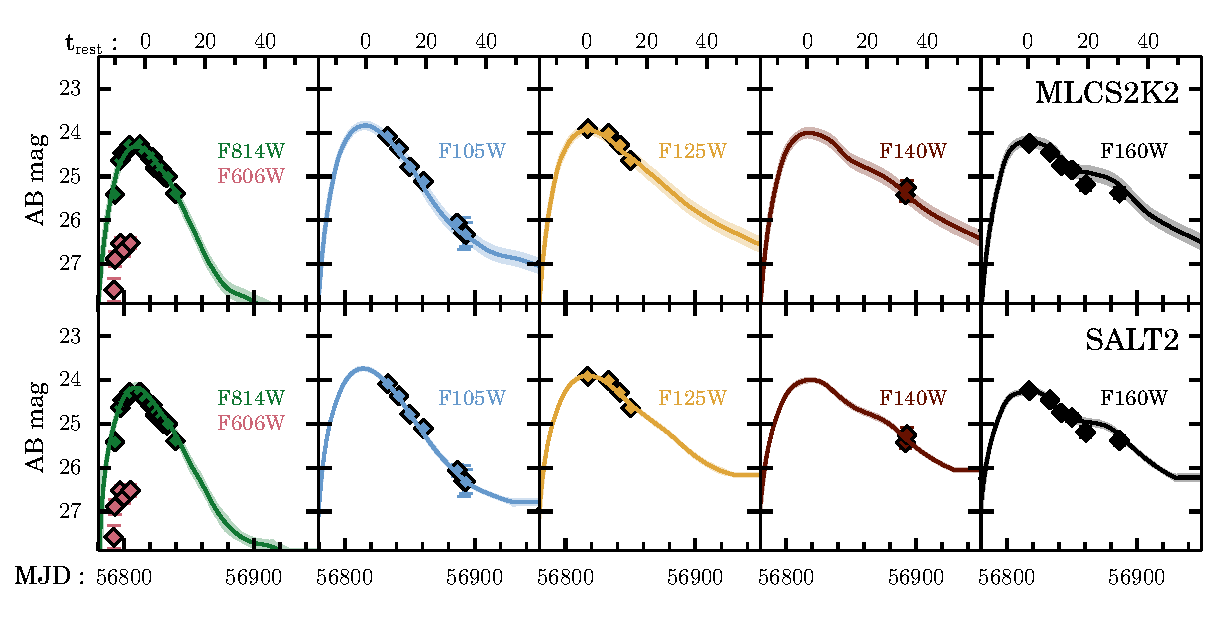
\includegraphics[width=0.8\textwidth]{FIG/snTomas_lightcurve_fit_magAB}
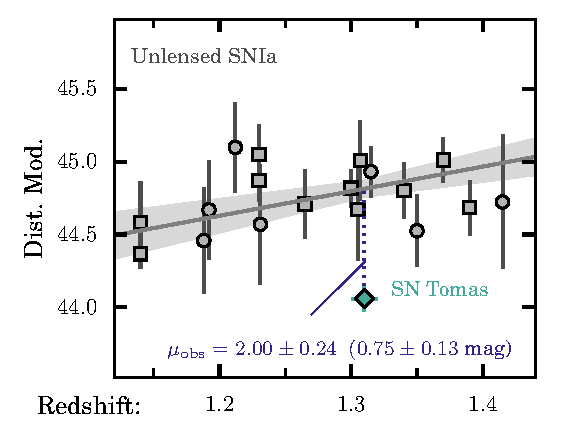
\includegraphics[width=0.55\textwidth]{FIG/snTomas_hubble_diagram}
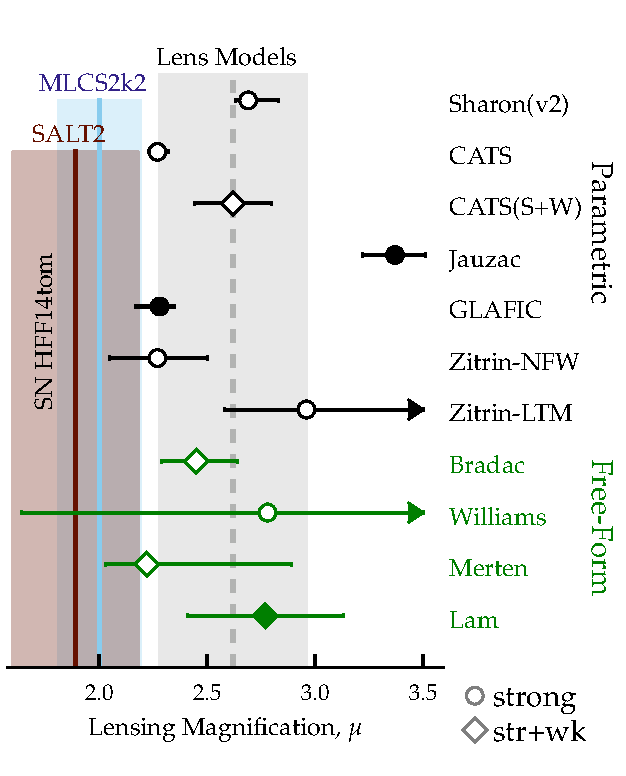
\includegraphics[width=0.44\textwidth]{FIG/snTomas_magnifications}%}
\caption{ \label{fig:tomas} \small
{\bf Testing Cluster Mass Models with Lensed \SNIa.}  SN HFF14tom is a
spectroscopically confirmed Type Ia SN at $z=1.33$, discovered by the
FrontierSN program behind the galaxy cluster Abell 2744 (z=0.308).
{\it(Left)} This SN is well matched by a normal \SNIa\ light curve
template with little extinction.  {\it(Center)} To define a
cosmology-independent ``true'' distance modulus, we use a linear fit
to the distances from un-lensed \SNe\ at similar
redshifts \citep{Riess:2007, Suzuki:2012}. The separation between the
best-fit line and our lensed SN gives us a measurement of the lensing
magnification with $\sim$10\% precision.  {\it (Right)} The vertical
gray bar indicates the measured magnification from the SN, and data
points show the predicted values from all publicly available lens
models. Collectively these models are {\it systematically
overestimating} the magnification. }
\end{figure*}


\pagebreak
\centerline {\bf Illuminating Dark Lenses with Highly Magnified Transients} 
\medskip

The FrontierSN program in Cycle 23 will also continue to discover
unique {\it strongly-lensed transients} behind the HFF clusters. Of
primary interest are lensed Type Ia SNe, with which we can directly
measure the true lensing magnification $\mu$ and confront the
predictions from existing lens models
\citep{Riehm:2011,Patel:2014,Nordin:2014}.  Figure~\ref{fig:tomas}
shows a Type Ia SN with a magnification
$\mu=2.00\pm0.19$ found in Cycle 21 \citep{Rodney:2015b}.  The
magnification of this SN is systematically {\it overestimated} by all
existing mass models, with some discrepant by $>5\sigma$.
{\bf Though small, our sample of lensed SNIa is already proving to be
  a very valuable tool for testing galaxy cluster dark matter models,}
which will be particularly valuable for the study of $z>8$ galaxies
magnified by these clusters
\citep[e.g.][]{Zheng:2012,Coe:2013,Bouwens:2014,Zitrin:2014}.

The unique combination of deep imaging, strong lensing, and rapid
cadence in the HFF program has also provided two very
exciting discoveries of {\it multiply-imaged} transients.  In January
and August of 2014, {\bf we observed two short transient events in
  separate images of the same strongly lensed galaxy at $z=1.0$.}
Collectively nicknamed ``Spock'', both of these events are too faint
to be a normal SN and too bright to be a stellar flare.  The light
curves are also faster than expected from a He shell explosion on a
white dwarf \citep[a ``.Ia'' event][]{Bildsten:2007,Shen:2010}, and
fainter than any of the ``fast optical transients'' yet seen in
wide-field ground-based surveys
\citep[e.g.][]{Kasliwal:2010,Poznanski:2010,Ofek:2010,Drout:2014,Vinko:2015}.

Lens models (and Occam's razor) suggest that these two events are most
likely {\it spatially coincident} on the source plane.  If the two
events were also {\it coincident in time}, then this could be an
example of an extremely rare neutron star collision \citep[a
  ``kilonova'';][]{Tanvir:2013,Kasen:2014,Metzger:2015}.  If not,
these may be two separate outbursts from an extremely bright nova with
a remarkably fast recurrence timescale of $\sim$1 year
(Figure~\ref{fig:spock}; Rodney et al., in prep).  This would be a
unique nova, as it would have a recurrence timescale on par with the
most extreme examples known \citep{Tang:2014} and would also be at
least an order of magnitude more luminous than a typical nova.

\begin{figure*}
%\vspace{-5mm}
\begin{center}
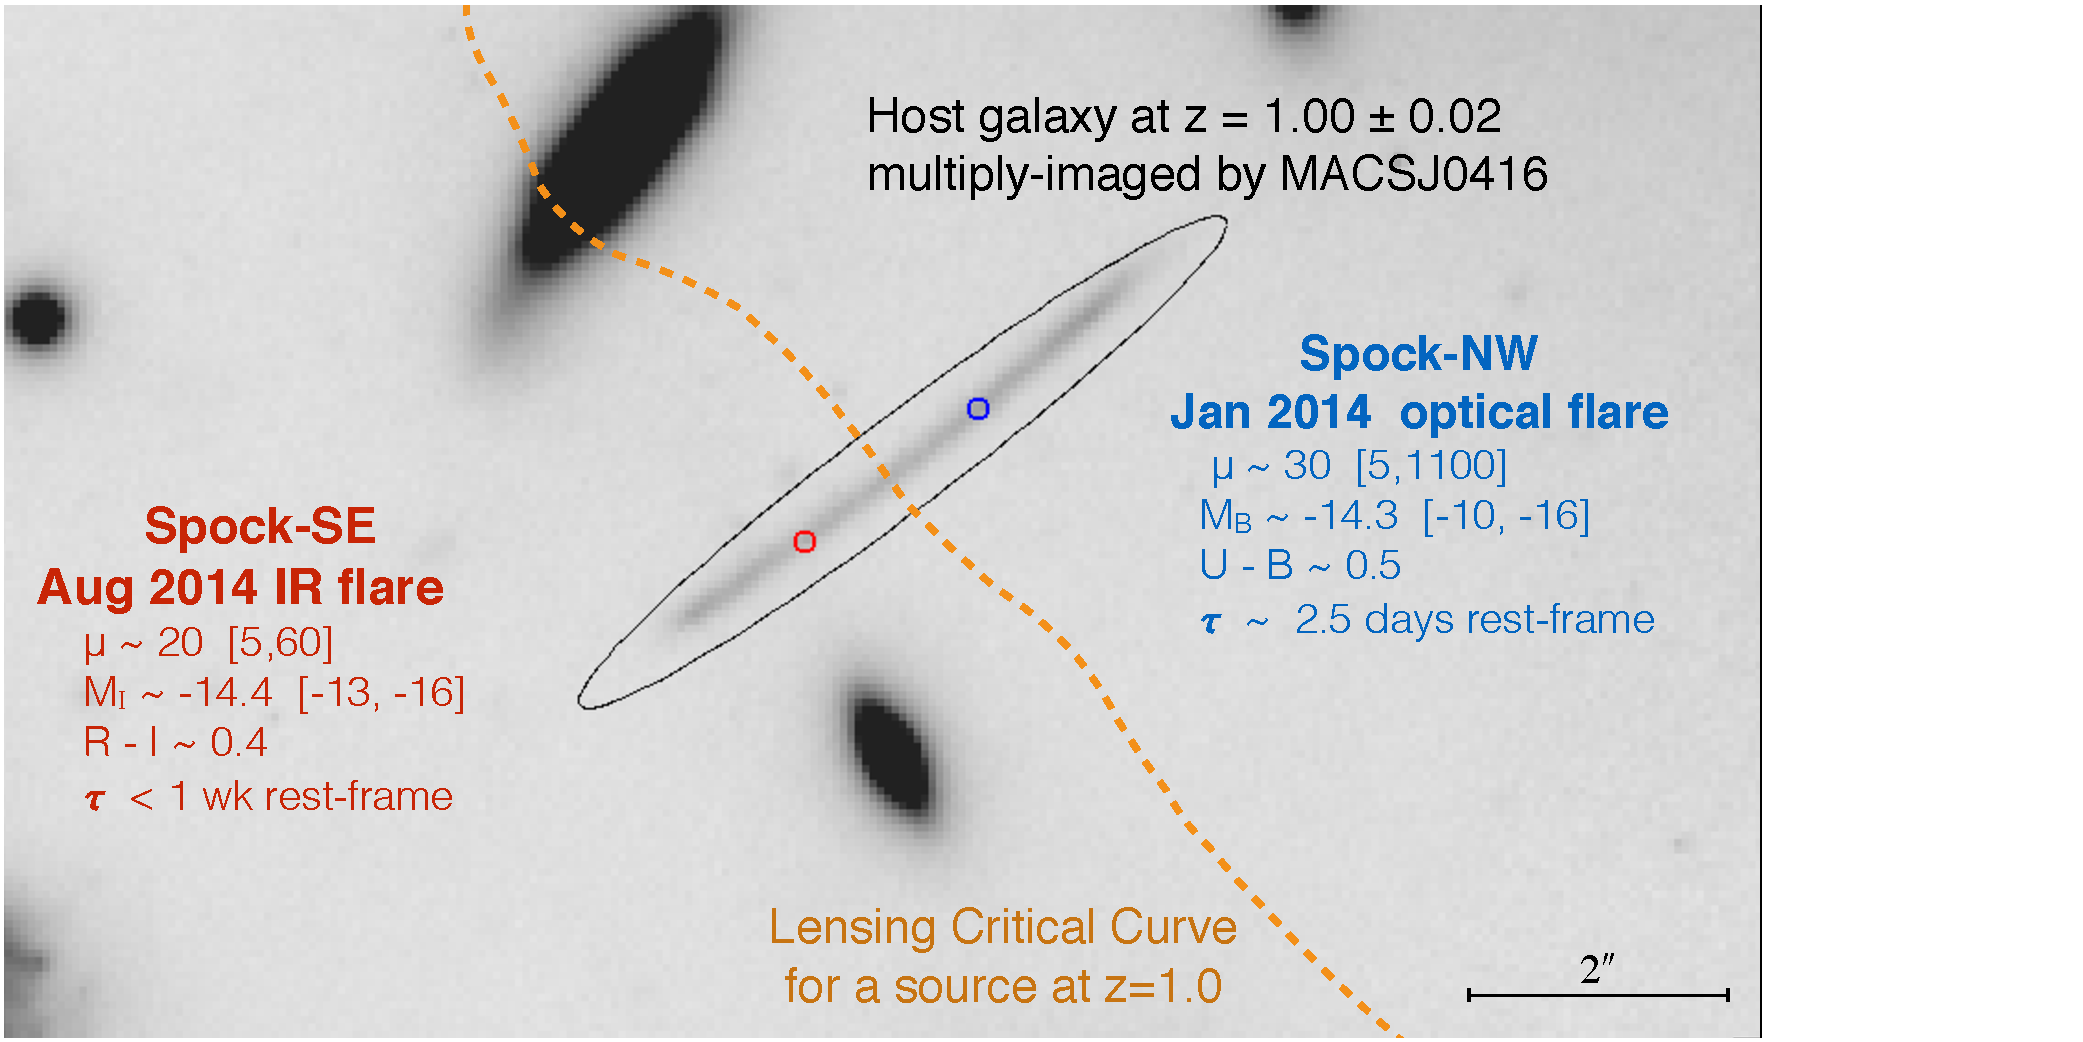
\includegraphics[width=0.63\textwidth]{FIG/spock_summary}
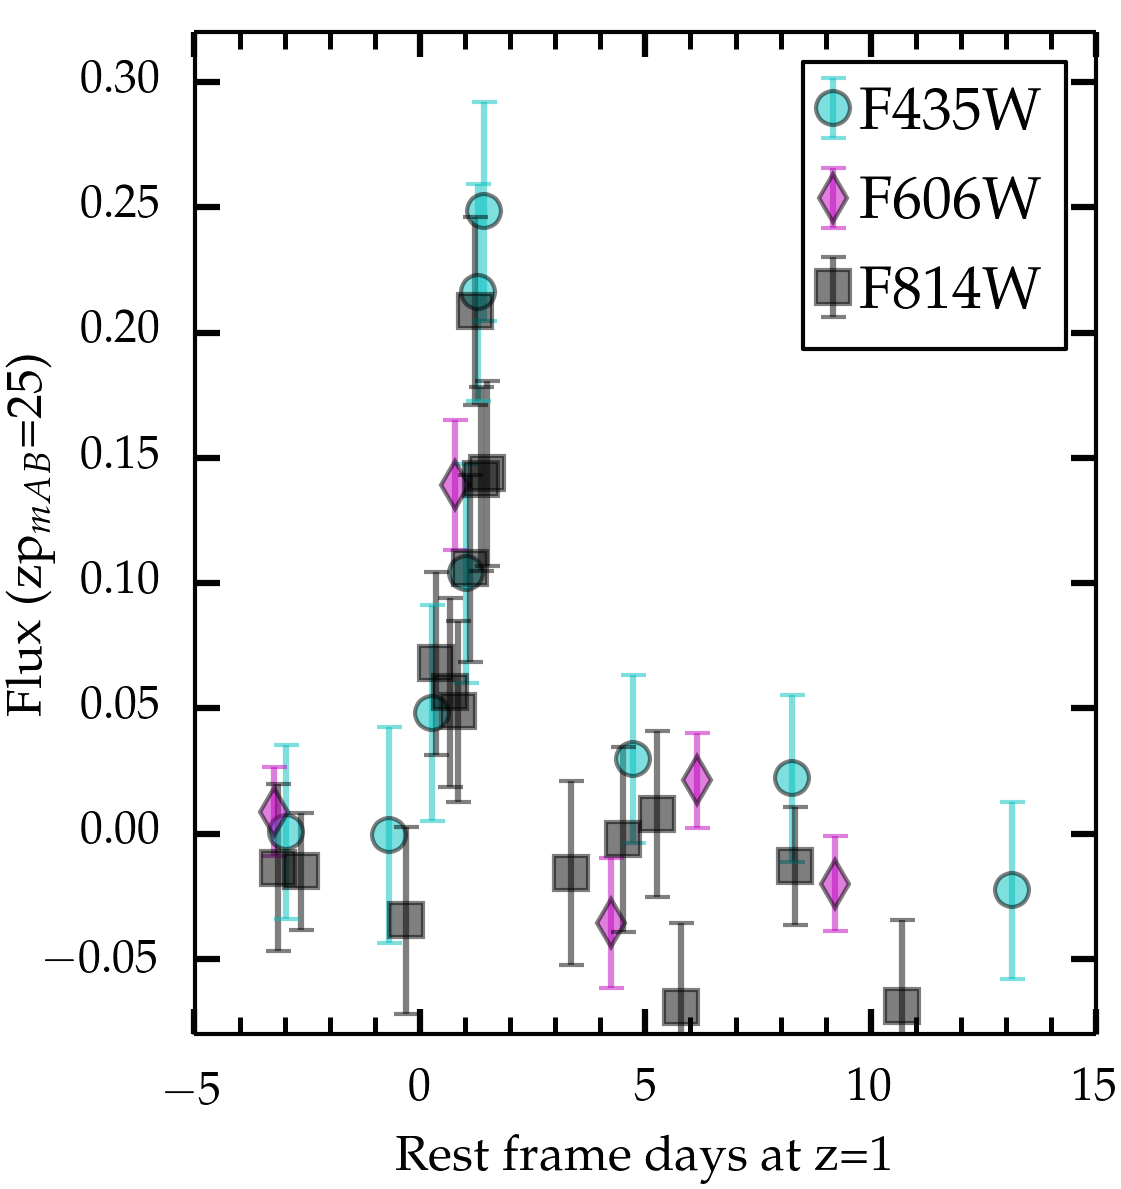
\includegraphics[width=0.36\textwidth]{FIG/spockNW_lightcurve_jan14event2}
\caption{ \label{fig:spock} %\small 
{\bf Spock, a peculiar pair of events.}  {\it Left:} A template
\HST\ image in the F814W band showing the locations of two transient
sources (nicknamed ``Spock-SE'' and ``Spock-NW'') that separately
appeared in adjacent images of a strongly-lensed galaxy at $z=1.0$
behind the Frontier Field cluster MACSJ0416. Lens models indicate that
a critical curve passes roughly mid-way between them, and they are
magnified by $\mu\sim20-30$ (3-4 mags).  {\it Right:} The light curve
of the Spock-NW event was captured in high-cadence HST-ACS imaging,
and the entire episode lasted only $\sim3$ rest-frame days. 
}
\vspace{3mm}
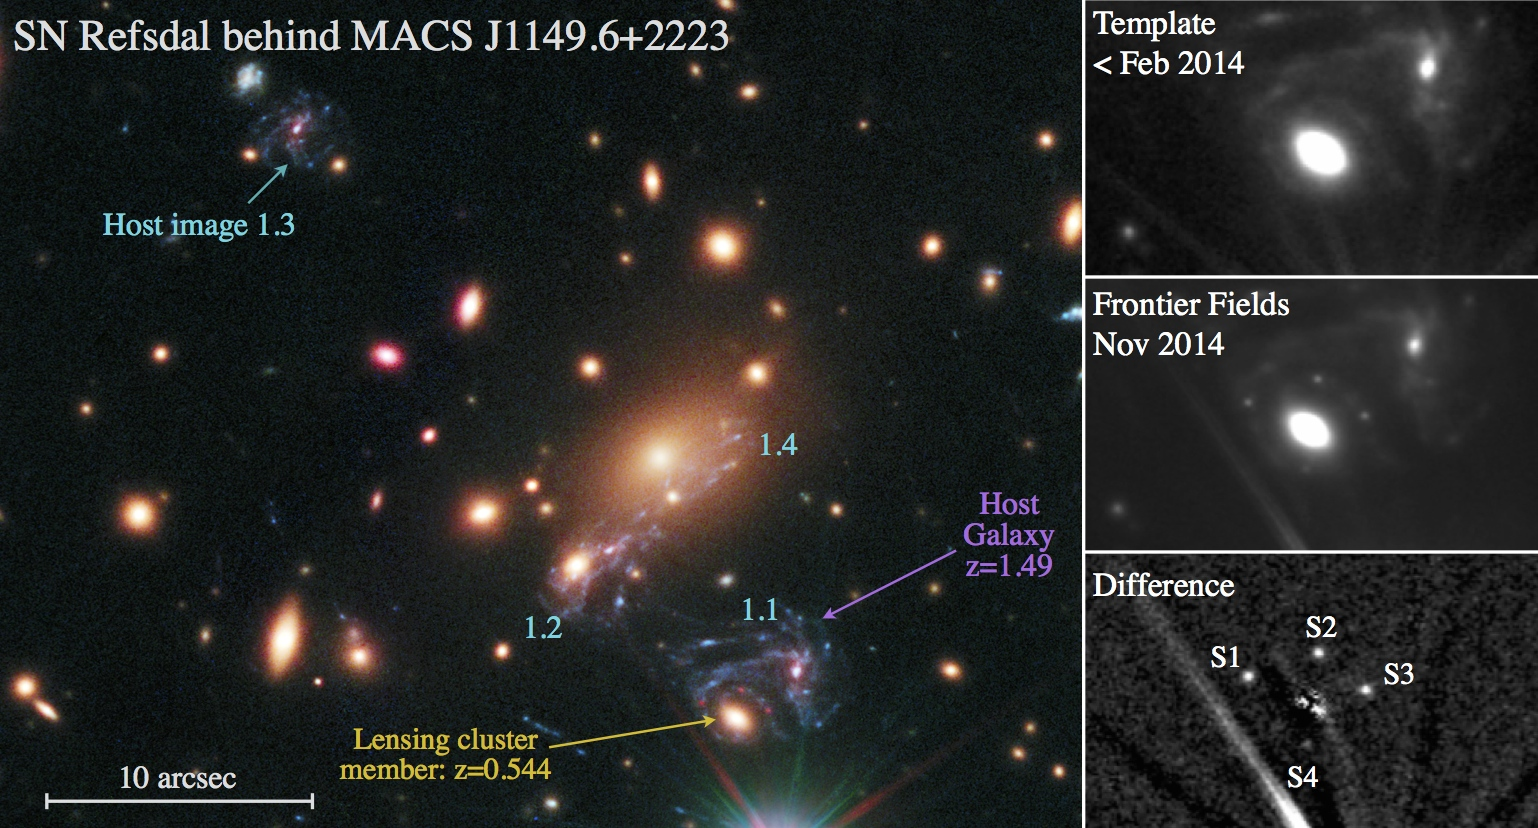
\includegraphics[width=0.88\textwidth]{FIG/refsdal_discovery.jpg}
 \caption{ %\small 
  {\bf Refsdal, the first multiply-imaged supernova.}
   The left panel shows a composite UV+optical+IR image of the central
   region of the galaxy cluster MACSJ1149 at $z=0.544$.  Cyan labels
   mark the locations of a multiply imaged face-on spiral galaxy at
   $z=1.49$.  The three panels at
   right partially enclose image 1.1 of this system, showing the
   appearance of 4 new point sources in WFC3-IR imaging collected in
   November, 2014 \citep{Kelly:2015}.
\label{fig:refsdal}  }
\end{center}
\end{figure*}

In November of 2014 we discovered another exciting transient, this
time with four distinct sources appearing $\sim$simultaneously in a
strongly lensed spiral galaxy at $z=1.5$.  Dubbed ``SN Refsdal,'' this
is the {\bf first ever example of a strongly lensed SN with multiple
  resolved images (Figure~\ref{fig:refsdal}; \citealt{Kelly:2015}).}
The Einstein Cross configuration shown in Figure~\ref{fig:refsdal} is
generated by a galaxy-scale lens, but the SN host galaxy is also
multiply imaged by the cluster, so {\bf we expect to see SN Refsdal
  return elsewhere in the cluster field in 1-5 years}
\citep{Oguri:2015,Sharon:2015}.  Measurements of the relative
magnifications and time delays among these multiple images will soon
deliver an unprecedented suite of powerful new mass model constraints.


%%%%%%%%%%%%%%%%%%%%%%%%%%%%%%%%%%%%%%%%%%%%%%%%%%%%%%%%%%%%%%%%%%%%%%%%%%%

%   2. DESCRIPTION OF THE OBSERVATIONS
%       (see Section 9.2 of the Call for Proposals)
%
%
\describeobservations   % Do not delete this command.
% Enter your observing description here.

In Cycle 23 the SN discoveries that this program will follow up will
come primarily from the HFF imaging of the final two cluster fields:
Abell 370 and Abell S1063. In addition, we are submitting a separate
Cycle 23 proposal (PI:Kelly) to provide regular monitoring of the
MACSJ1149 field with HST imaging.  That Cycle 23 program is needed to
measure time delays between the 4 images of SN Refsdal
(Figure~\ref{fig:refsdal}) and catch it's predicted reappearance).  If
that MACSJ1149 program is approved, it will effectively provide a
third SN survey field in Cycle 23. Our FrontierSN team will search
for any {\it new} SNe, lensed or otherwise, that appear in the
MACSJ1149 cluster field or the associated parallels.

Based on our simulations of the HFF survey and the actual yield in the
first two years, we expect to find another 8-12 SNe in Cycle 23, with
uncertainty dominated by poisson statistics for the small number of
events in any single survey year.  As our first two years have shown,
it is extremely difficult to prognosticate the actual number of orbits
that will be required for effective follow-up of this final-year HFF
SN sample.  Using the first two years as a guide, {\bf we request a new
allocation  of 20 orbits for Cycle 23.}

We anticipate spending $\sim$6 orbits on 2-5 candidate SNe that might
be at high redshift ($z>1$) or significantly magnified ($\mu>2$).  The
deep and frequent HFF imaging visits will provide a high S/N and
well-sampled light curve in either ACS optical bands or WFC3 IR bands.
Our follow-up imaging will provide the complementary bands needed for
optical-NIR colors, which are critical for photometric classification
and redshift estimation of $z>1$ SNe \citep{Riess:2004a,Rodney:2012}.
A typical target in this category might have an AB magnitude of 26.5,
requiring a single-orbit visit to get 2-3 filters from the same
camera.  In some cases multiple epochs of observations are warranted
to improve the classification and redshift estimate.

We expect the other $\sim$14 orbits will be devoted to one or two
objects of particular interest: very high redshift ($z>1.5$) and/or
strongly lensed ($\mu>5$) transients like SN \tomas, SN Refsdal, and
Spock.  These orbits will be used for optical/IR imaging or grism
spectroscopy, as appropriate for the source redshift and class.  As an
example, SN \tomas\ at $z=1.3$ reached a peak brightness at $\sim24$
AB mag in IR bands, and we followed the light curve down to 26.2 AB mag
in F140W.  The total cost of follow-up was 11 orbits: 5 orbits for ACS
G800L grism and 6 single-orbit visits to collect the rest-frame
optical light curve using WFC3-IR broad bands.


%Of the 20 transient sources discovered in GLASS imaging data, we added
%additional observations on 6 objects, using 13 orbits.  The other 21
%orbits were expended following 4 out of the 18 transients found in HFF
%imaging.  This would have left us with $\sim$26 orbits for follow-up
%of any SNe found during the remainder of Cycle 22 and in the two final
%HFF fields observed during Cycle 23.



%%%%%%%%%%%%%%%%%%%%%%%%%%%%%%%%%%%%%%%%%%%%%%%%%%%%%%%%%%%%%%%%%%%%%%%%%%%

%   3. SPECIAL REQUIREMENTS
%       (see Section 9.3 of the Call for Proposals)
%
%
\specialreq             % Do not delete this command.
% Justify your special requirements here, if any.


This SN follow-up program requires ToO status, and we request 5
non-disruptive ToO triggers for the cycle.  Most of our SN targets
that warrant follow-up observations are at $z>1$, with significant
time dilation, and the deep Frontier Field imaging typically provides
early detections for many of them.  Therefore the non-disruptive time
delay of 3 weeks is acceptable for all our triggers.

We additionally request a continuation of the fast-ftp delivery of our
FrontierSN observations immediately after those data become available,
as has been implemented for our program in Cycles 21 and 22.  Rapid
delivery and analysis allows us to respond to new information from our
follow-up observations and adjust future visits without requiring
disruptive ToO's.

Recognizing the special nature of the Frontier Fields, and the value
of early community access to transient data, we request no proprietary
period for our ToO follow-up observations.


%%%%%%%%%%%%%%%%%%%%%%%%%%%%%%%%%%%%%%%%%%%%%%%%%%%%%%%%%%%%%%%%%%%%%%%%%%%

%   4. COORDINATED OBSERVATIONS
%       (see Section 9.4 of the Call for Proposals)
%
%
\coordinatedobs          % Do not delete this command.
% Enter your coordinated observing plans here, if any.


When possible, we will choose the orient of our follow-up orbits such
that the parallel camera (ACS or WFC3) falls back onto the Frontier
Field footprint.  In those cases we will use filters optimized for SN
discovery, providing additional SN search epochs.  When such an orient
is not available, we will consult with the Frontier Field team at
STScI to provide the most useful parallel observations (e.g. for
improving cluster weak lensing constraints).


%%%%%%%%%%%%%%%%%%%%%%%%%%%%%%%%%%%%%%%%%%%%%%%%%%%%%%%%%%%%%%%%%%%%%%%%%%%

%   5. JUSTIFY DUPLICATIONS
%       (see Section 9.5 of the Call for Proposals)
%
%
\duplications           % Do not delete this command.
% Enter your duplication justifications here, if any.

This program is essentially a resubmission of an approved multi-cycle
ToO program from Cycle 21 (PI:Rodney, PID:13386,13790). The proposal
in Cycle 21 anticipated a total sample of $\sim$20 SNe over 3 years,
requiring 60 orbits of HST Target of Opportunity (ToO) follow-up
observations.  This forecast was based on the expected yield from the
HFF survey alone.  The approval of the GLASS program in Cycle 21
roughly doubled the effective survey volume, and as GLASS had no
dedicated HST follow-up resources, we have used our FrontierSN orbits
to follow the GLASS discoveries as well.

We have used {\bf 34 orbits} from our FrontierSN allocation for follow-up
imaging and spectroscopy of 10 transient candidates found in the GLASS
and HFF survey imaging.  Of these 34 orbits, half were spent on just
two objects of interest, SN Tomas (Figure~\ref{fig:tomas}) and Spock
(Figure~\ref{fig:spock}).  This was in keeping with our initial
expectations in the Cycle 21 FrontierSN proposal, where we anticipated
roughly half of our 60-orbit allocation would be spent on such
high-impact objects.

However, our predictions for HST follow-up needs were shattered by the
unprecedented discovery of the multiply-imaged SN Refsdal.  To
classify this SN and confirm its redshift, we acquired a new
allocation of 36 orbits for HST grism spectroscopy and optical imaging
through a director's discretionary program.  It was also necessary to
commit another {\bf 24 orbits} from our FrontierSN program for IR
imaging to collect the SN light curve, which enables a measurement of
the gravitational lensing time delay.  This leaves us with only 2
orbits left for follow-up of any SNe found in the remaining 5 months
of HFF imaging in Cycle 22, plus the entirety of Cycle 23.


%%%%%%%%%%%%%%%%%%%%%%%%%%%%%%%%%%%%%%%%%%%%%%%%%%%%%%%%%%%%%%%%%%%%%%%%%%%


%   6. PAST HST USAGE
%       (see Section 9.8 of the Call for Proposals)
%
%        List here the program numbers and data status for all accepted GO/AR/SNAP 
%        programs of the PI in at least the last four HST Cycles. Include a list of refereed publications 
%        resulting from these programs.       
%
%       Note that the description of past HST usage  DOES NOT count against the page limits of the proposal.
%
\pasthstusage  % Do not delete this command.

% List here the program numbers and data status for all accepted GO/AR/SNAP
% programs of the PI in at least the last four HST Cycles. Include a list of refereed
% publications resulting from these programs.

Table\,\ref{tab:pasthstusage} lists the HST programs from recent cycles that include PI Rodney.

\begin{deluxetable}{p{0.25\linewidth}p{0.15\linewidth}p{0.2\linewidth}p{0.3\linewidth}}
%\rotate
\tablecolumns{4}
\tablecaption{Past HST Usage for PI \label{tab:pasthstusage}}
\tablehead{   \colhead{PID}  & \colhead{Title} & \colhead{Status} & 
  \colhead{Selected Publications\tablenotemark{*}} }
\startdata
12060-64, 12440-45 & CANDELS & Cycle 18-20 MCT;\linebreak complete. & \citealt{Grogin:2011}\linebreak \citealt{Trump:2011}\linebreak \citealt{van-der-Wel:2011} \\[6pt]
12065-69, 12100-04, 12451-60 & CLASH & Cycle 18-20 MCT;\linebreak complete. & \citealt{Postman:2012}\linebreak \citealt{Coe:2013}\\[22pt]
12099, 12461, 13063 & C+C SN Follow-up & Cycle 18-20 MCT;\linebreak complete. & \citealt{Rodney:2012}\linebreak \citealt{Frederiksen:2012}\linebreak \citealt{Jones:2013}\linebreak \citealt{Graur:2014}\linebreak \citealt{Rodney:2014}\linebreak \citealt{Rodney:2015a}\\[6pt]
13046 & RAISIN & Cycle 20 ToO;\linebreak complete & \nodata \\[22pt]
13386,13790 & FrontierSN & Cycle 21-23 ToO;\linebreak precursor to this proposal & \citealt{Kelly:2015}\linebreak \citealt{Rodney:2015b}\\

\enddata
\tablenotetext{*}{Listed publications are those with direct input from PI Rodney and the CANDELS+CLASH SN team. Total CANDELS+CLASH publications $\approx$63.}
\end{deluxetable}

%%%%%%%%%%%%%%%%%%%%%%%%%%%%%%%%%%%%%%%%%%%%%%%%%%%%%%%%%%%%%%%%%%%%%%%%%%%
%  Bibliography goes in before or after PAST HST usage ??
%  Probably before, since it has to be counted in the text page limit
%%%%%%%%%%%%%%%%%%%%%%%%%%%%%%%%%%%%%%%%%%%%%%%%%%%%%%%%%%%%%%%%%%%%%%%%%%%

%\smallskip
\newpage
\setlength{\bibsep}{-2pt}
\begin{spacing}{0.5}
\bibliographystyle{apjbrief}
{\footnotesize
\bibliography{bibdesk}
}
\end{spacing}




%%%%%%%%%%%%%%%%%%%%%%%%%%%%%%%%%%%%%%%%%%%%%%%%%%%%%%%%%%%%%%%%%%%%%%%%%%%

\end{document}          % End of proposal. Do not delete this line.
                        % Everything after this command is ignored.

